% Copyright 2023 The terCAD team. All rights reserved.
% Use of this content is governed by a CC BY-NC-ND 4.0 license that can be found in the LICENSE file.

\subsection{Benchmarking Prototype} \label{benchmark}
\markboth{Unleashing}{Benchmarking Prototype}

Before adding muscle functionality to the created prototype skeleton, we must verify its reliability. Restructuring the 
application's fundamental concepts in the future would pose considerable challenges and entail substantial effort and 
potential complications.


\subsubsection{Providing Integration Tests} \label{int-tests}

Unit (\ref{ut-unit}) and widget (\ref{widget-tests}) tests are valuable tools for assessing isolated classes, functions, 
or widgets. However, they cannot address all problems. Integration tests identify systemic flaws, such as data 
corruption, concurrency problems, and miscommunication between services, that might not be evident in unit tests. They 
do this by verifying the synergy of individual assets. Integration tests validate the application as a whole. They are 
designed to reflect the real-time performance of an application on an actual device or platform. In conclusion, they 
provide a vital link in the testing hierarchy by validating the collaboration of various components within an 
application. In this way, integration tests simulate the end-to-end user workflows we implemented and discussed earlier 
(see \ref{t-gherkin}).

Flutter integration tests can be written using the \q{integration\_test}-package. In addition, the \q{flutter\_driver} 
package helps us evaluate tests on real or virtual devices and environments, and track the timeline of test execution. 
Both packages are provided by the SDK.

\begin{lstlisting}[language=yaml]
## ./pubspec.yaml
dev_dependencies:
  integration_test:
    sdk: flutter
  flutter_driver: 
    sdk: flutter
\end{lstlisting}

\noindent The implementation differs from a widget test in its use of the following code line, which enables test 
execution on a physical device or platform:

\begin{lstlisting}
IntegrationTestWidgetsFlutterBinding.ensureInitialized();
\end{lstlisting}

\noindent \q{Firebase Test Lab} and \q{BrowserStack} are cloud-powered testing platforms that enable evaluation of integration tests across an extensive spectrum of devices and configurations.

Note that Just-In-Time (JIT) and Ahead-of-Time (AOT) compilers (see \ref{dart}) may produce different results. What 
works flawlessly in development mode (JIT) may not work as well in release mode (AOT), as demonstrated by the following 
image \cref{img:compilation-err}. This is why integration tests are valuable in the automated verification process.

\img{features/compilation-err}{Deviation between JIT (left) and AOT (right) compilations}{img:compilation-err}

\subsubsection{Doing Performance Testing}

Performance testing is a type of software testing that evaluates an application's speed, responsiveness, stability, and 
overall performance under different conditions. It involves subjecting the application to simulated workloads and stress 
scenarios to evaluate its behavior in terms of speed, scalability, and resource usage. Through performance testing, 
developers can ensure that the software can handle the expected load without experiencing a degradation in performance.

Performance testing simulates different levels of user traffic to help determine an application's scalability. It does 
this by assessing resource utilization (CPU, memory, network bandwidth, etc.) and identifying performance bottlenecks, 
such as slow database queries, inefficient code, or network latency. Addressing these issues before they impact users is 
crucial.

Detailed information about performance testing can be found in the International Software Testing Qualifications Board (ISTQB) or the Software Engineering Institute (SEI) publications. Here, we will only highlight their definitions
(\cite{Ian15}, \cite{Sag16}, \cite{Sag23}):
\begin{itemize}
  \item Load Testing: Evaluates how an application performs under expected load conditions. It helps determine the 
  application's response time, resource utilization, and overall stability.

  \item Stress Testing: Pushes the application to its limits by subjecting it to extreme conditions, such as excessive 
  user loads or resource scarcity. It aims to identify the breaking point and understand how the application recovers 
  from failures.

  \item Endurance Testing: Assesses the application's performance over an extended period to identify issues related to 
  memory leaks, resource exhaustion, or gradual degradation in performance.

  \item Spike Testing: Simulates sudden spikes in user traffic to assess how the application responds to rapid changes
  in load. This helps uncover bottlenecks and issues related to sudden surges in demand.

  \item Volume Testing: Focuses on testing the application's performance with large volumes of data, such as a high 
  number of records in a database. It helps identify scalability and performance issues associated with data volume.
\end{itemize}

\noindent Returning to our process, the following command would be used to evaluate performance tests:

\begin{lstlisting}[language=terminal]
# Precondition for Web profiling
chromedriver --port=4444
# Launch tests
flutter drive \
  --driver=test_driver/perf_driver.dart \
  --target=integration_test/name_of_test.dart \
  --profile
\end{lstlisting}

\noindent The \q{--profile}-option enables application compilation in "profile mode," which helps benchmark results 
reflect the experience of end users. When running on a mobile device or emulator, it is recommended to use the 
\q{--no-dds}-parameter, which disables the inaccessible Dart Development Service (DDS). The \q{--target}-option declares 
the scope of test executions, and the \q{--driver}-option tracks the outcomes. The driver configuration can be found at 
\href{https://docs.flutter.dev/cookbook/testing/integration/profiling}{https://docs.flutter.dev/cookbook/testing/integration/profiling}:

\begin{lstlisting}
// ./test_driver/perf_driver.dart
import 'package:flutter_driver/flutter_driver.dart' as driver;
import 'package:integration_test/integration_test_driver.dart';

Future<void> main() {
  return integrationDriver(
    responseDataCallback: (data) async {
      if (data != null) {
        final timeline = driver.Timeline.fromJson(data['timeline']);
        final summary = driver.TimelineSummary.summarize(timeline);
        await summary.writeTimelineToFile(
          'timeline',
          pretty: true,
          includeSummary: true,
          destinationDirectory: './coverage/',
        );
      }
    },
  );
}
\end{lstlisting}

\noindent Since it's a Widget Tests-based approach (\ref{widget-tests}, \ref{t-gherkin}), we'll focus only on using the 
\q{traceAction}-method to store time-based metrics:

\begin{lstlisting}
// ./test/performance/load/creation_test.dart
void main() {
  final binding = IntegrationTestWidgetsFlutterBinding.ensureInitialized();

  testWidgets('Cover Starting Page', (WidgetTester tester) async {
    await binding.traceAction(() async {
        // ... other steps
        final amountField = find.byWidgetPredicate((widget) {
          return widget is TextField && 
              widget.decoration?.hintText == 'Set Balance';
        });
        await tester.ensureVisible(amountField);
        await tester.tap(amountField);
        // In profiling mode some delay is needed:
        await tester.pumpAndSettle(const Duration(seconds: 1));
        // await tester.pump();
        await tester.enterText(amountField, '1000');
        await tester.pumpAndSettle();
        expect(find.text('1000'), findsOneWidget);
        // ... other steps
      },
      reportKey: 'timeline',
    );
  });
}
\end{lstlisting}

\noindent Generated \q{timeline.timeline.json}-file can be traced by \q{chrome://tracing/} in Google Chrome browser 
(\cref{img:perf-chrome-tracing}):

\img{features/perf-chrome-tracing}{Google Chrome -- performance trace}{img:perf-chrome-tracing}

\noindent The \q{timeline.timeline\_summary.json}-file is a native \q{JSON}-file that can be opened in an IDE for manual 
inspection. However, it is mostly used in CI/CD to fail the build if any defined parameter is outside the specified 
range. For example, the recommended value for the \q{average\_frame\_build\_time\_millis}-parameter is below 16 
milliseconds to ensure the app runs at 60 frames per second without glitches. Other parameters are described in detail 
on the page 
\href{https://api.flutter.dev/flutter/flutter\_driver/TimelineSummary/summaryJson.html}{https://api.flutter.dev/flutter/flutter\_driver/TimelineSummary}.


\subsubsection{Measuring Responsiveness}
\paragraph{Load Testing}

Check the response time and resource utilization for the initial setup by creating an account and budget category:

\begin{lstlisting}[language=cucumber]
@start
Feature: Verify Initial Flow
  Scenario: Applying basic configuration through the start pages
    Given I am firstly opened the app
    Then I can see "Initial Setup" component
    When I tap "Save to Storage (Go Next)" button
    Then I can see "Acknowledge (Go Next)" component
    When I tap "Acknowledge (Go Next)" button
    Then I can see "Create new Account" component
    When I tap on 0 index of "ListSelector" fields
    And I tap "Bank Account" element
    And I enter "New Account" to "Enter Account Identifier" text field
    And I enter "1000" to "Set Balance" text field
    And I tap "Create new Account" button
    Then I can see "Create new Budget Category" component
    When I enter "New Budget" to "Enter Budget Category Name" text field
    And I enter "1000" to "Set Balance" text field
    When I tap "Create new Budget Category" button
    Then I can see "Accounts, total" component
\end{lstlisting}

\noindent From executions (see \cref{tb:frame-build}), we've identified a degraded frame build parameter that affects 
our frames per second (FPS) by generating only 37 frames instead of 60:\\

\begin{table}[h!]
  \begin{tabular}{ |p{6.8cm}||r|r|r|  }
    \hline
    \multicolumn{4}{|c|}{Frame Build Time, in milliseconds} \\
    \hline
    Type of state & Cold Start & Retrial & With Data\\
    \hline
    average          &  26.00 &  24.28 &  29.65 \\
    90th percentile  &  47.20 &  43.38 &  70.33 \\
    99th percentile  & 158.31 & 159.41 & 198.03 \\
    \hline
  \end{tabular}
  \caption{Performance Test Results for Feature "Verify Initial Flow"} \label{tb:frame-build}
\end{table}

\img{features/perf-slow-frame}{Performance Monitor in Visual Studio Code}{img:perf-slow-frame}

\noindent This issue (see figure \cref{img:perf-slow-frame}) relates to janky animations caused by shader calculations. 
Shaders are code snippets executed on a graphics processing unit (GPU) to render a sequence of draw commands. The 
pre-compilation strategy mitigates disruptions related to compilation during subsequent animations and improves 
rendering of frames per second. To run the app with \q{--cache-sksl} turned on to capture shaders in SkSL:

\begin{lstlisting}[language=terminal]
$ flutter run --profile --cache-sksl --purge-persistent-cache
\end{lstlisting}

\noindent During the build, warm up shaders in Skia Shader Language (SkSL) format:

\begin{lstlisting}[language=terminal]
# Capture shaders in Skia Shader Language (SkSL) format into a file
$ flutter drive --profile --cache-sksl \
  --write-sksl-on-exit sksl.json -t test_driver/warm_up.dart
# Build app with SkSL warm-up
$ flutter build ios --bundle-sksl-path sksl.json
\end{lstlisting}

\begin{lstlisting}
// ./test_driver/warm_up.dart
Future<void> main() => integrationDriver();(*@ \stopnumber @*)

// ./test_driver/warm_up_test.dart
Future<void> main() async {
  IntegrationTestWidgetsFlutterBinding.ensureInitialized();
  SharedPreferencesMixin.pref=await SharedPreferences.getInstance();
  testWidgets('Warm-up', (WidgetTester tester) async {
    await tester.pumpWidget(MultiProvider(
      providers: [
        ChangeNotifierProvider<AppData>(create: (_) => AppData()),
        ChangeNotifierProvider<AppTheme>(
          create: (_) => AppTheme(ThemeMode.system),
        )],
      child: const MyApp(),
    ));
    await tester.pumpAndSettle(const Duration(seconds: 3));
  });
\end{lstlisting}

\noindent We've achieved an average of 56 FPS through SkSL caching alone, but there are many other factors that 
contribute to responsiveness optimization.

Further enhancements can be achieved by optimizing listeners like \q{MediaQuery.of(content)}. This is because its usage 
can inadvertently result in extensive rebuilds, especially when the keyboard is toggled between the shown and hidden 
states. This is due to the intrinsic behavior of the \q{.of(context)} listeners, which react to any change, including 
updates to the MediaQuery's \q{viewInsets} property. This can trigger all the \q{.of(context)} listeners, even if they 
don't use the aforementioned property, which ultimately affects performance. The solution is partial listening in 
Flutter: \q{MediaQuery.platformBrightnessOf} for brightness and \q{MediaQuery.sizeOf} to track height and width. This 
simple tweak provides substantial benefits to application performance.

Another avenue for enhancement lies in converting functions involving widget generation into native widgets. This aims 
to optimize resource consumption and caching mechanisms. Flutter's tendency to preload all UI components and then feed 
data to existing widgets during runtime makes this approach beneficial. This approach circumvents the need to rebuild 
the entire dynamic UI from scratch in a single frame as necessitated by function callbacks:

\begin{lstlisting}
// Not recommended
ListView.builder(
  itemCount: 5000,
  itemBuilder: (BuildContext context, int index) {
    return _getMyWidget(); // Function call
  }
);
// Better option
ListView.builder(
  itemCount: 5000,
  itemBuilder: (context, int index) => const MyWidget()
);
\end{lstlisting}

\noindent Optimizing the use of \q{StatefulWidget} has the potential to improve performance, primarily because fewer 
widgets control the lifecycle. This streamlined approach translates to faster response times.

The \q{RepaintBoundary}-widget can be used for render decoupling, which isolates parts that need to be repainted from 
the rest of the tree. The child widget will then be rendered independently of its parent widget. Constantly animated 
widgets, for example, can be wrapped by a \q{RepaintBoundary}-widget to prevent the rest of the UI from being 
unnecessarily repainted.

The \q{AutomaticKeepAliveClientMixin}-mixin is another solution for retaining the state of expensive widgets or widgets 
that come in and out of view, such as \q{ListView} and \q{GridView}, by preserving the state of nested 
\q{StatefulWidget}s.

\begin{lstlisting}
@override
bool get wantKeepAlive => true;
\end{lstlisting}

\noindent The same flow can almost be achieved by using the \q{Offstage}-widget, which toggles the visibility of its 
children without removing them from the widget tree (and mostly without losing their state or triggering a rebuild).

It is not obvious, but it can be acknowledged that the Flutter upgrade procedure (for example, upgrading to Flutter 3.10 
can triple the frame rate if the background color of the \q{FlutterViews} is changed to a non-nil value, as cited in 
\cite{Chis23}). Conversely, the upgrade itself can lead to outages due to broken dependencies and missing package 
support:

\begin{lstlisting}[language=terminal]
[!] CocoaPods could not find compatible versions for 
  pod "flutter_webrtc"

[!] `<XCBuildConfiguration name=`Debug` UUID=`...`>` attempted to 
  initialize an object with an unknown UUID `...` for attribute: 
  `base_configuration_reference`. This can be the result of a 
  merge and the unknown UUID is being discarded.
\end{lstlisting}


\subsubsection{Anticipating Churn Rate}

\paragraph{Volume Testing} Check the initial load, which is the amount of time before the interaction is enabled, with a 
huge transaction log history (32 MB, 128 MB, 512 MB, or 2 GB).

In this test, our main goal is to accurately measure how long it takes for the main page to become fully accessible to 
users. To achieve this, we will continuously monitor the application's state, focusing particularly on the disappearance 
of the "Project Initialization" header. This monitoring process enables us to identify the moment when the application 
becomes responsive and ready for user interaction. 

To gain a comprehensive perspective, we supplement the elapsed time measurement with an analysis of the transaction log 
history. By correlating loading time with log size, we can identify potential performance bottlenecks or issues related 
to the application's initialization process.

\begin{lstlisting}
// ./integration_test/stress/initialization_test.dart
testWidgets('Cover Initial Page', (WidgetTester tester) async {
  await _init(tester); // Start app by using 'pumpWidget'
  FileRunner.tester = tester;
  await FirstRun().executeStep(); // verify that data is loaded
  // Change test execution timeout
}, timeout: const Timeout(Duration(minutes: 30)));
\end{lstlisting}
\begin{lstlisting}
// ./test/e2e/_steps/given/first_run.dart
class FirstRun extends Given with SharedPreferencesMixin {
  @override
  RegExp get pattern => RegExp(r"I am firstly opened the app");

  @override
  Future<void> executeStep() async {
    Finder init;
    do {
      init = find.text('Project Initialization');
      await FileRunner.tester.pumpAndSettle(const Duration(microseconds: 50));
    } while (init.evaluate().isNotEmpty);
    await FileRunner.tester.pumpAndSettle();
  }
}
\end{lstlisting}

\begin{figure}
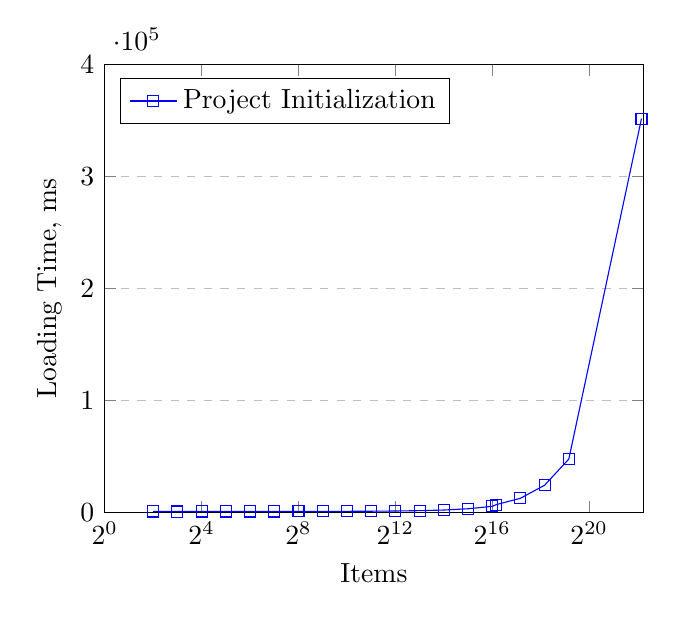
\begin{tikzpicture}
  \begin{axis}[
    xlabel={Items},
    ylabel={Loading Time, ms},
    xmin=0, xmax=5000000,
    ymin=0, ymax=400000,
    xmode=log,
    log basis x={2},
    legend pos=north west,
    ymajorgrids=true,
    grid style=dashed,
  ] 
  \addplot[
    color=blue,
    mark=square,
    ]
    coordinates {
      (0, 863) (4, 935) (8, 887) (16, 937) (32, 931) (64, 932) (128, 957) (256, 1014) (512, 1025) (1024, 1069) 
      (2048, 1169) (4096, 1358) (8192, 1664) (16384, 2221) (32768, 3351) (65536, 5515) (73659, 7064) (146444, 12687)
      (292888, 24353) (585776, 47693) (4686208, 351456)
    };
    \legend{Project Initialization}
  \end{axis}
\end{tikzpicture}
\caption{Stress Testing: Loading Time vs. Number of Items} \label{t-stress}
\end{figure}

\noindent The results (see \cref{t-stress}) have shown that the time required for a cold start varies from 863 
milliseconds with zero items to 5.85 minutes to load a 2.53 GB log file containing 4.7 million items. This is far from 
our assertion of less than two seconds for the current solution with an 8.20 MB file size and 16,400 items. This implies 
that after consistent usage for one and a half to five years, our customers may encounter a situation in which opening 
the application takes longer than two seconds. Based on the retrieved data, we must optimize initialization by 
implementing a warm-up caching strategy, also known as hot, warm, and cold caches \cite{Tom17}.


\paragraph{Endurance Testing}

Check the response time and resource utilization by adding different types of data over different time periods (15 
minutes, one hour, four hours, and eight hours).

For that test, we would like to debug memory issues using DevTools. DevTools is a suite of performance and debugging 
tools for Dart and Flutter. It can be started from an IDE with the necessary extensions installed by pressing \key{F1} 
and typing \q{devtools}.

Detecting memory leaks involves analyzing the heap snapshot from the Memory View tab. These snapshots 
(\cref{img:memory-snapshot}) provide a means of comparing heap growth and identifying objects that might increase in 
number unexpectedly. Although images and media can contribute substantially to memory consumption, they are often not 
the root cause of memory leaks. Instead, attention should be directed toward addressing the incomplete rebound 
phenomenon (see \cref{img:memory-leak}) for resident set size (RSS), which is the program's memory currently loaded into 
RAM and available for immediate use. One example of a large, short-lived object that could inadvertently enter a 
long-lived area and lead to leaks is the \q{context}-parameter transmitted to Flutter's build method:

\begin{lstlisting}
Widget build(BuildContext context) {
\end{lstlisting}
{
\xpretocmd{\lstlisting}{\vspace{-12pt}}{}{}
\begin{lstlisting}[firstnumber=2, backgroundcolor=\color{backred}]
(*@\kdiff{-}@*)  // [!] Leak prone issue
(*@\kdiff{-}@*)  final handler = () => apply(Theme.of(context));
\end{lstlisting}
\begin{lstlisting}[firstnumber=2, backgroundcolor=\color{backgreen}]
(*@\kdiff{+}@*)  final theme = Theme.of(context);
(*@\kdiff{+}@*)  final handler = () => apply(theme);
\end{lstlisting}
\begin{lstlisting}[firstnumber=4]
   useHandler(handler);
\end{lstlisting}
}

\img{features/memory-snapshot}{DevTools: Heap Snapshot within the Memory View}{img:memory-snapshot}
\img{features/memory-leak}{Incomplete rebound phenomenon for RSS}{img:memory-leak}
\img{features/devtools-connection}{DevTools: Connect to the running instance}{img:devtools-connection}

\noindent To track the CPU and memory heap, we'll run DevTools separately and connect it 
(\cref{img:devtools-connection}) to the process via the URL provided in the output of the integration tests:

\begin{lstlisting}[language=terminal]
Building Windows application...           13.1s
V  Built build\windows\runner\Debug\Fingrom.exe.
VMServiceFlutterDriver: Connecting to Flutter application at 
    http://127.0.0.1:52135/VDm4NX0QVr4=/
\end{lstlisting}

\noindent The test itself will simulate a user behavior by randomly creating bills (90\%), budget categories (10\%), 
and accounts (5\%): 

\begin{lstlisting}
testWidgets('Imitate User Activities', (WidgetTester tester) async {
  final startTime = DateTime.now();
  await cleanUp();
  await firstRun(tester);
  Duration duration;
  int idx = 0;
  final r = Random();
  do {
    if (r.nextDouble() <= 0.05) await createAccount(tester, idx);
    await FileRunner.tester.pumpAndSettle(const Duration(seconds: 5));
    if (r.nextDouble() <= 0.10) await createBudget(tester, idx);
    await FileRunner.tester.pumpAndSettle(const Duration(seconds: 5));
    if (r.nextDouble() <= 0.90) await createBill(tester, idx);
    await FileRunner.tester.pumpAndSettle(const Duration(seconds: 5));
    final endTime = DateTime.now();
    duration = endTime.difference(startTime);
    idx++;
  } while (duration.inMinutes < 15);
}, timeout: const Timeout(Duration(hours: 9)));
\end{lstlisting}

\noindent After a couple minutes of execution, an error occurred:

\begin{lstlisting}[language=terminal]
Running scenario: Create new Bill # :2
  V Given I am on "Home" page # :3 took 945ms
  V When I tap "Add Bill, Income or Transfer" button # :4 took 356ms
  V And I tap on 0 index of "ListAccountSelector" fields # :5 took 696ms
  V And I tap on 0 index of "BaseLineWidget" fields # :6 took 350ms
  V And I tap on 0 index of "ListBudgetSelector" fields # :7 took 465ms
  V And I tap on 0 index of "BaseLineWidget" fields # :8 took 350ms
  V And I enter "10" to "Set Amount" text field # :9 took 266ms
  V And I enter "Bill #8" to "Set Expense Details" text field
RangeError (index): Invalid value: Valid value range is empty: -1
\end{lstlisting}

\noindent The problem is linked to a guarded function conflict (the first method had not finished executing when the 
second one was called), as well as a \q{tap}-action on buttons that leads to \q{Navigator.pop} or \q{Navigator.push} 
execution. It can be "easily" resolved by adding a duration freeze and making assertions synchronous (changing 
\q{expect} to \q{expectSync}):

\begin{lstlisting}
// ./test/e2e/_steps/when/tap_defined_button.dart
final btn = find.byTooltip(name);
await FileRunner.tester.ensureVisible(btn);
expectSync(btn, findsOneWidget);
await FileRunner.tester.tap(btn);
await FileRunner.tester.pumpAndSettle(Duration(milliseconds: 400));
\end{lstlisting}

\noindent As a result of investigating that case, a couple of problems have been noticed. One of them relates to a 
missing initial record in the transaction logs:

\begin{lstlisting}[language=terminal]
FormatException: Invalid length, must be multiple of four
\end{lstlisting}

\noindent The problem is that the transaction log file was created with a BOM as the first character on a line, which is 
why encryption is failing. Good catch! Let's insert a new line when the file is created and proceed. Additionally, there 
was a problem with \q{FloatingActionButton}-buttons:

\begin{lstlisting}[language=terminal]
The following assertion was thrown during a scheduler callback:
  There are multiple heroes that share the same tag within a subtree.
  Within each subtree for which heroes are to be animated (i.e. a 
  PageRoute subtree), each Hero must have a unique non-null tag.
  In this case, multiple heroes had the following tag: 
    <default FloatingActionButton tag>
\end{lstlisting}

\noindent The error indicates that there are multiple \q{Hero}-widgets (\q{FloatingActionButton}-buttons, in our case) 
with the same tag within a subtree. In Flutter, Heroes are used to create smooth animations when transitioning between 
screens or widgets. Each Hero widget must have a unique, non-null tag to properly manage animation between source and 
destination widgets. Therefore, we must make them unique by adding a \q{heroTag}-property to each \issue{130}{b4369fc}.

Lastly, our exhaustive endurance testing revealed memory leaks during intensive application usage, as shown in 
\cref{img:memory-profiler}. In short, each new interaction with the application impacts its responsiveness, resulting in 
noticeable performance degradation after a few minutes, as shown in \cref{gr:taken-cycle} "Initial State". This fix must 
be implemented before any other changes, as ignorance would result in a loss of users who would have a negative first 
impression. By analyzing DevTools traces, we identified the source of the problem. The fix resulted in a 1 ms gain at 
the start without any significant forecast degradation over time (see \cref{img:m-profiler-after} and 
\cref{gr:taken-cycle} "Adjusted").

\img{features/memory-profiler}{Flutter DevTools: Memory Profiler Results}{img:memory-profiler}
\img{features/memory-profiler-after}{Flutter DevTools: Memory Profiler Results after Refactoring}{img:m-profiler-after}

\begin{figure}
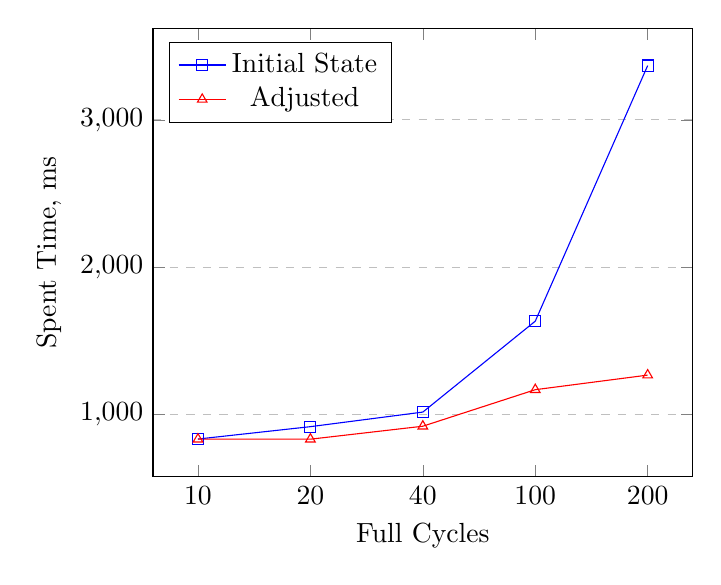
\begin{tikzpicture}
  \begin{axis}[
    title={},
    xlabel={Full Cycles},
    ylabel={Spent Time, ms},
    legend pos=north west,
    ymajorgrids=true,
    grid style=dashed,
    xtick=data,
    xticklabels={10, 20, 40, 100, 200},
  ]
  \addplot[
    color=blue,
    mark=square,
    ]
    coordinates {
    (1, 833) (2, 917) (3, 1016) (4, 1633) (5, 3368)
    };
    \addlegendentry{Initial State}
  
    \addplot[
      color=red,
      mark=triangle,
      ]
      coordinates {
      (1, 832) (2, 832) (3, 920) (4, 1168) (5, 1267)
      };
      \addlegendentry{Adjusted}
  \end{axis}
\end{tikzpicture}
\caption{Taken Cycles of Items Creation vs. Spent Time} \label{gr:taken-cycle}
\end{figure}
